\documentclass[10pt, a4paper,spanish]{article}

\usepackage{./mystyle}
\usepackage{./myvars}



%-----------------------------

\begin{document}

	\maketitle % Insert title

	\thispagestyle{fancy} % All pages have headers and footers


%-----------------------------
%	ABSTRACT
%-----------------------------

	\begin{abstract}
		\noindent Abstract
	\end{abstract}

%-----------------------------
%	TEXT
%-----------------------------

	\setcounter{section}{4}

	\section{Construir el árbol de decisión según el algoritmo \emph{ID3}, calculando todas las ganancias a la hora de escoger el siguiente atributo}

		\begin{table}[h]
			\begin{center}
				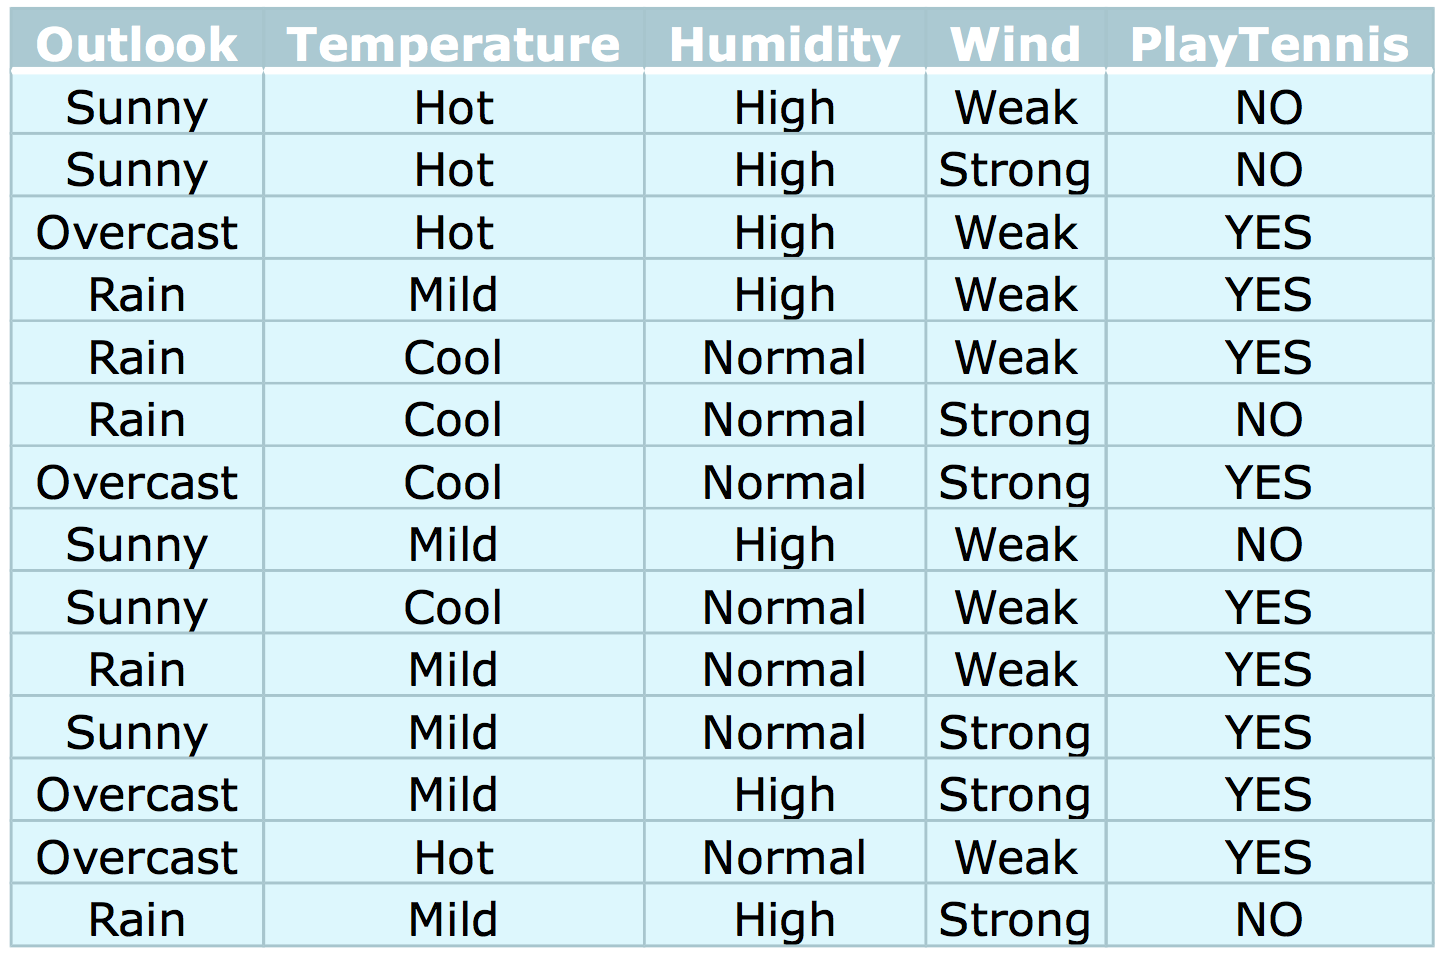
\includegraphics[width=0.5\textwidth]{table-exercise-4}
				\caption{Datos para el algoritmo \emph{ID3}}
			\end{center}
			\label{e4:table}
		\end{table}

		\paragraph{}
		El algoritmo \emph{ID3} consiste en un generador de árboles de decisión. Los árboles de decisión son estructuras jerárquicas utilizadas para resolver problemas de clasificación mediante técnicas de aprendizaje automático. En este caso, el algoritmo se basa en aprendizaje supervisado, es decir, en el periodo de aprendizaje utiliza un conjunto de datos en el cuál el valor de destino de la clasificación está fijado previamente.

		\paragraph{}
		El aprendizaje basado en árboles de decisión utiliza la generación de estructuras en forma de árbol etiquetado. Un árbol etiquetado consiste en un grafo $G$ no dirigido que posee las siguientes propiedades\cite{wiki:tree}:

 		\begin{itemize}
			\setlength\itemsep{0em}
 			\item $G$ es conexo y no tiene ciclos.
			\item $G$ no tiene ciclos y, si se añade alguna arista se forma un ciclo.
			\item $G$ es conexo y si se le quita alguna arista deja de ser conexo.
			\item $G$ es conexo y el grafo completo de 3 vértices $K_{3}$ no es un menor de $G$.
			\item Dos vértices cualquiera de $G$ están conectados por un único camino simple.
			\item Cada arista posee una etiqueta con la cuál se identifica.
 		\end{itemize}

		\paragraph{}
		En el contexto del aprendizaje, dichos árboles representan lo siguiente:

		\begin{itemize}
			\setlength\itemsep{0em}
			\item Los vértices internos representan atributos de los datos
			\item El proceso de clasificación comienza por el vértice padre del arbol (vértice sin padre).
			\item Las aristas etiquetadas representan el valor que toma el atributo, de tal manera que si el dato toma el valor fijado por la etiqueta de la arista en el atributo fijado en el vértice padre, entonces el próximo atributo a inspeccionar es el que representa el vértice hijo al cual se llega a partir de dicha arista.
			\item Los vértices hoja (vértices sin hijos) representa los valores que toman el valor de la clase en la cual será clasificado el dato.
 		\end{itemize}

		\paragraph{}
		Para la generación del árbol de decisión existen varias heurísticas, en el caso del algoritmo \emph{ID3} la intuición utilizada se basa en la disciplina de la teoría de información, que a grandes rasgos consiste en buscar recursivamente el atributo que mayor relación tenga con el valor esperado de la clase para dicho dato. Además se apoya en los conceptos de \textbf{Información}, \textbf{Entropía} y \textbf{Ganancia de Información}, los cuales se describen a continuación: Sea $S = \{ S_1, S_2, S_q \}$ el conjunto de valores discretos que puede tomar un determinado atributo y $P(S_i)$ la probabilidad de ocurrencia de dicho valor.

		\begin{equation}
			\label{eq:information}
			I(S_i) = \log \frac{1}{P(S_i)}
		\end{equation}

		\paragraph{}
		En la equación \eqref{eq:information} se describe la cantidad de información que proporciona un determinado valor $S_i$ del conjunto $S$ de posibles valores que puede tomar el dato.

		\begin{equation}
			\label{eq:entropy}
			H(S) = \sum_{i=1}^q P(S_i)I(S_i)
		\end{equation}

		\paragraph{}
		La equación \eqref{eq:entropy} describe la entropia de un atributo, esto puede traducirse como una medida de la cantidad de infomación que se puede obtener de un atributo $S$. La idea en que se basa esto consiste en la intuición de que si el conjunto de valores está uniformemente distribuido en su rango, la entropía del mismo tomará valores más altos, lo cuál hará que probablemente ese atributo sea más valioso para la clasificación si este está relacionado con la clase como se describe a continuación. En cambio, si la distribución de valores que toma el atributo está muy concentrada, probablemente este atributo suministrará un menor grado de información por lo que su entropía es menor.


		\begin{equation}
			\label{eq:ganancy}
			G(S, A) = H(S) - \sum_{i=1}^k \frac{\mid S_{v_i} \mid }{ \mid S \mid }H(S_{v_i})
		\end{equation}

		\paragraph{}
		La ganancia de información se define en la equación \eqref{eq:ganancy}. Esta es la medida que utiliza la heurística en que se basa el algoritmo de generación de árboles \emph{ID3}. Dicha equación proporciona el grado de relación entre un atributo $A$ del conjunto de datos y la clase $S$ en que se desean clasificar los mismos.

		\paragraph{}

		\begin{algorithm}
			\emph{ID3} utiliza la equación \eqref{eq:ganancy} para generar un ránking con los atributos del conjunto de datos, seleccinando el de mayor ganancia respecto de la clase como vértice padre y creando tantas aristas como valores no vaciós tome dicho atributo. Repite este proceso por cada una de las aristas de forma recursiva eliminando el atributo selecionado y filtrando los datos de entrenamiento a las especificaciones fijadas por el camino seguido, hasta que todos los datos toman un único valor, en cuyo caso crea un vértice hoja con dicho valor, la disyunción de valores de la clase si se eliminan todos los atributos o \emph{desconocido} si no hay datos suficientes para continuar el proceso
		\end{algorithm}

		\paragraph{}
		Para el cálculo de resultados se ha realizado una implementación en el lenguaje \emph{Python} la cual calcula el ranking citado anteriormente. Dicha implementación se puede visualizar a través de la ruta \url{https://github.com/garciparedes/python-examples/blob/master/machine_learning/utils/gainranking.py}\cite{github:garciparedes-python-examples}. Además, se ha realizado una implementación básica de la generación del árbol de decisión mediante \emph{ID3} la cual se puede visualizar en \url{https://github.com/garciparedes/python-examples/blob/master/machine_learning/decision_tree/id3.py}\cite{github:garciparedes-python-examples}


		\paragraph{}
		En este caso, el conjunto de datos se muestra en la tabla \ref{e4:table}. Está formado por un conjunto de 4 atributos, además del valor esperado de la clase. Todos ellos toman valores discretos, por lo que no es necesario realizar discretizaciones, lo cual se ajusta perfectamente a la entrada esperada del Algoritmo \emph{ID3}. La clase se corresponde con el atributo \textbf{PlayTennis}. A continuación se describe una ejecución paso a paso del algoritmo.

		\begin{table}[H]
			\centering
			\begin{tabular}{| c | c |}
				\hline
	 			Atributo 			& Ganancia \\ \hline
				Outlook 			& 0.246750 \\ \hline
				Humidity 			& 0.151836 \\ \hline
				Wind 					& 0.048127 \\ \hline
				Temperature 	& 0.029223 \\ \hline
			\end{tabular}
			\caption{ID3 sobre el conjunto de datos: Paso 1}
			\label{e4:algorithm-step1}
		\end{table}

		\begin{table}[H]
			\centering
			\begin{tabular}{| c | c |}
				\hline
				Atributo 			& Ganancia \\ \hline
				Humidity 			& 0.970951 \\ \hline
				Temperature 	& 0.570951 \\ \hline
				Wind 					& 0.019973 \\ \hline
			\end{tabular}
			\caption{ID3 sobre el conjunto de datos: Paso 2}
			\label{e4:algorithm-step2}
		\end{table}

		\begin{table}[H]
			\centering
			\begin{tabular}{| c | c |}
				\hline
				Atributo 			& Ganancia \\ \hline
				Wind 					& 0.970951 \\ \hline
				Humidity 			& 0.019973 \\ \hline
				Temperature 	& 0.019973 \\ \hline
			\end{tabular}
			\caption{ID3 sobre el conjunto de datos: Paso 3}
			\label{e4:algorithm-step3}
		\end{table}

		\begin{figure}[h]
			\begin{center}
				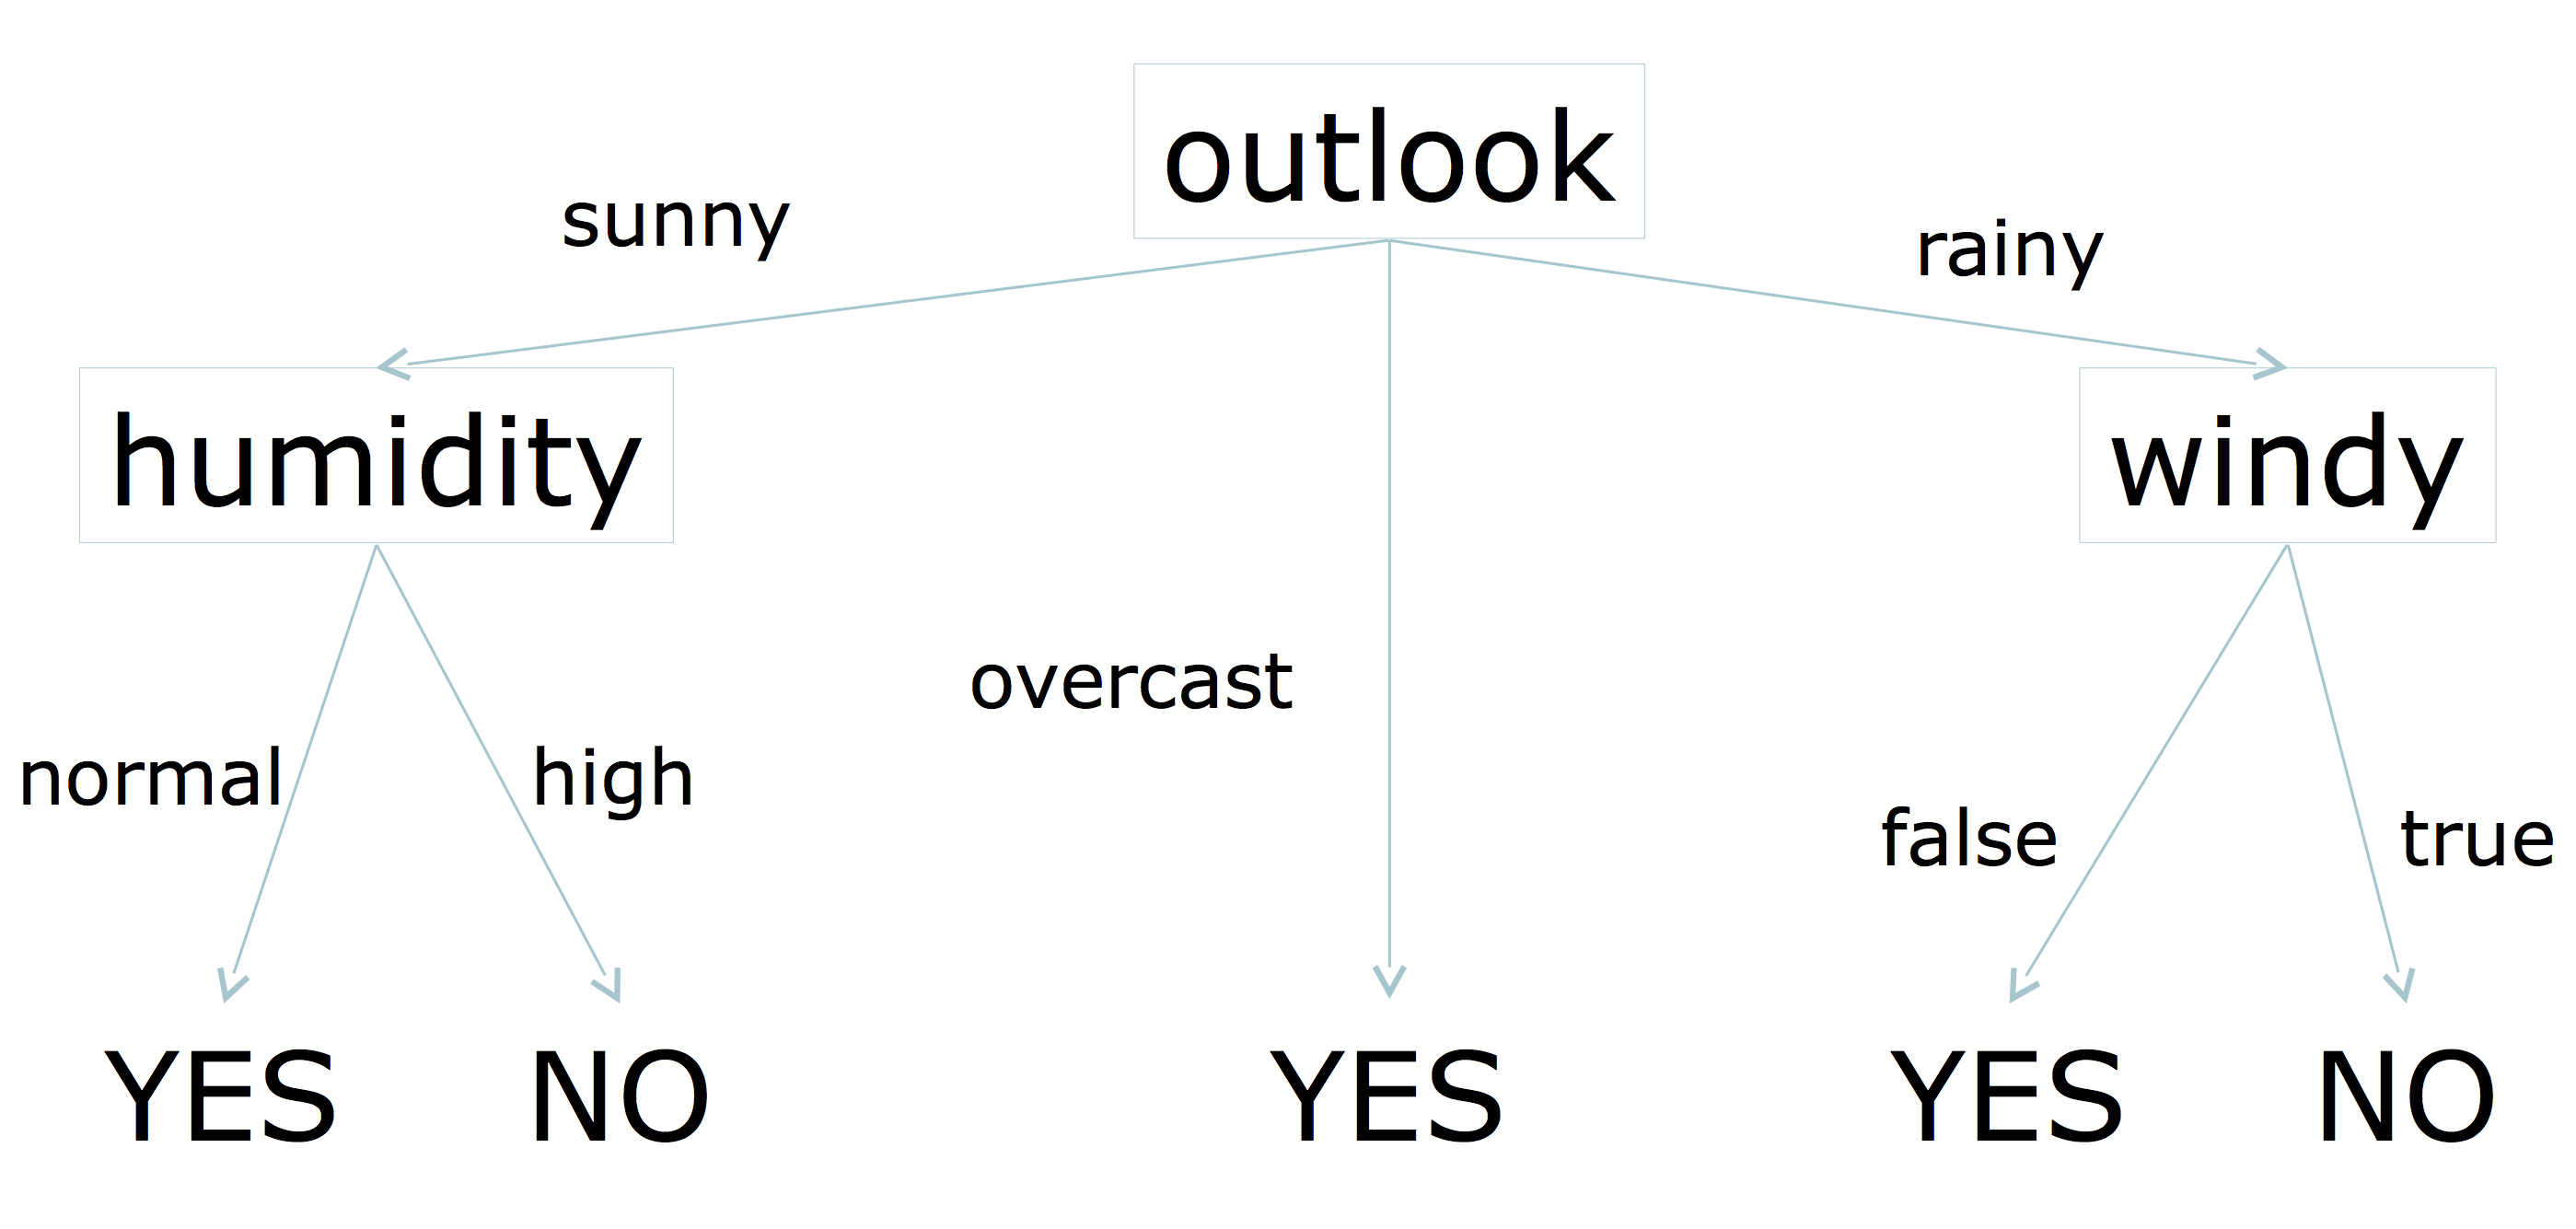
\includegraphics[width=0.7\textwidth]{tree-exercise-4}
				\caption{Árbol resultante tras ejecutar el algoritmo \emph{ID3} \cite{subject:taa}}
			\end{center}
			\label{e4:tree}
		\end{figure}

		\paragraph{}
		El en las tablas \ref{e4:algorithm-step1}, \ref{e4:algorithm-step2} y \ref{e4:algorithm-step3} se muestran los resultados de los rankings de ganancia en cada paso del algoritmo \emph{ID3} implementado en \emph{Python} tal y como se cita anteriormente. El árbol resultante de la ejecución coincide con el presentado en las diapositivas de la asignatura \cite{subject:taa} y se muestra en la figura \ref{e4:tree}.



	\section{Calcular las siguientes ganancias en este ejemplo de 6 muestras}

		\begin{table}[h]
			\begin{center}
				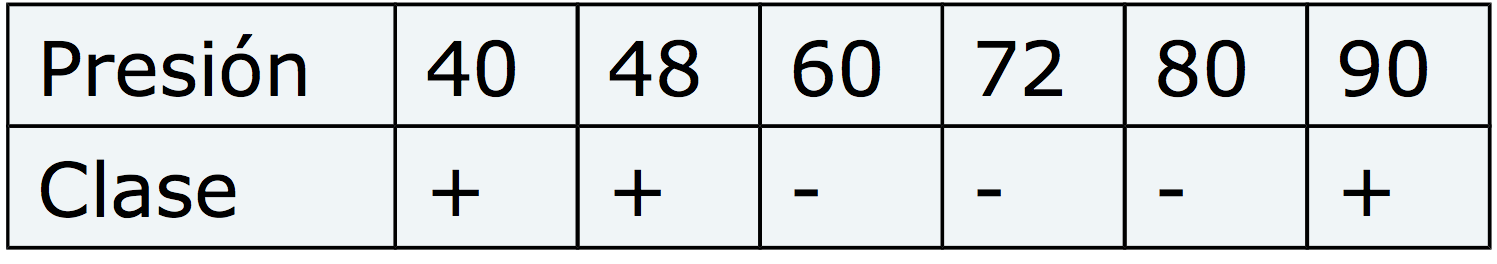
\includegraphics[width=0.3\textwidth]{table-exercise-5}
				\caption{Datos para cálculo de ganancias}
			\end{center}
			\label{e5:table}
		\end{table}

		\paragraph{}
		Se pide calcular las ganancias resultantes trás discretizar el atributo \emph{Presión} de la tabla \ref{e5:table} mediante su particionado en los puntos $c_1 = 54$ y $c_2 = 85$. Denotaremos por $S$ al atributo de la clase. Lo siguiente es calcular su entropía tal y como se ha hecho en la equación \eqref{eq:e5-class-entropy}

		\begin{equation}
			\label{eq:e5-class-entropy}
			H(S) = \frac{2}{6}\log(\frac{6}{2}) + \frac{4}{6}\log(\frac{6}{4}) = 0.636514...
		\end{equation}

		\paragraph{}
		A continuación se muestra el número de instancias asociadas a cada clase para después calcular la ganancia de información obtenida tras dicha discretización a través de las equaciones \eqref{eq:e5-h1less},  \eqref{eq:e5-h1more} y \eqref{eq:e5-g1}.

		\begin{itemize}
			\setlength\itemsep{0em}
			\item $A_{c_1} = \{ +, - \}$
			\item $A_{c_1 <} \leftarrow \{ 2+, 0- \}$
			\item $A_{c_1 >} \leftarrow \{ 1+, 3- \}$
		\end{itemize}

		\begin{equation}
			\label{eq:e5-h1less}
			H(A_{c_1 <}) = \frac{2}{2}\log(\frac{2}{2}) + \frac{0}{2}\log(\frac{2}{0}) = 0.0
		\end{equation}

		\begin{equation}
			\label{eq:e5-h1more}
			H(A_{c_1 >}) = \frac{1}{4}\log(\frac{4}{1}) + \frac{3}{4}\log(\frac{4}{3}) = 0.562335...
		\end{equation}

		\begin{equation}
			\label{eq:e5-g1}
			G(S, A_{c_1}) = 0.636514... - (\frac{2}{6} * 0.0 + \frac{4}{6} * 0.562335...) = 0.261624...
		\end{equation}

		\paragraph{}
		A continuación se muestra el número de instancias asociadas a cada clase para después calcular la ganancia de información obtenida tras dicha discretización a través de las equaciones \eqref{eq:e5-h2less},  \eqref{eq:e5-h2more} y \eqref{eq:e5-g2}:

		\begin{itemize}
			\setlength\itemsep{0em}
			\item $A_{c_2} = \{ +, - \}$
			\item $A_{c_2 <} \leftarrow \{ 2+, 3- \}$
			\item $A_{c_2 >} \leftarrow \{ 1+, 0- \}$
		\end{itemize}

		\begin{equation}
			\label{eq:e5-h2less}
			H(A_{c_2 <}) = \frac{2}{5}\log(\frac{5}{2}) + \frac{3}{5}\log(\frac{5}{3}) = 0.673011...
		\end{equation}

		\begin{equation}
			\label{eq:e5-h2more}
			H(A_{c_2 >}) = \frac{1}{1}\log(\frac{1}{1}) + \frac{0}{1}\log(\frac{1}{0}) = 0.0
		\end{equation}

		\begin{equation}
			\label{eq:e5-g2}
			G(S, A_{c_2}) = 0.636514... - (\frac{5}{6} * 0.673011... + \frac{1}{6} * 0.0) = 0.0756715...
		\end{equation}

		\paragraph{}
		Puesto que la \textbf{Ganancia de Información} obtenida tras la partición por $c_1 = 54$ es significativamente mayor a la obtenida por $c_2 = 85$ debido a que $G(S, A_{c_1}) = 0.261624... > G(S, A_{c_2}) = 0.0756715...$, el particionamiento se realiza en el punto \textbf{$c_1$}.

	\section{aplicar el algoritmo J48 al ejemplo anterior modificado, en el que se detallan valores numéricos de la temperatura. Explique el resultado del árbol resultante frente a la temperatura}

		\begin{table}[h]
			\begin{center}
				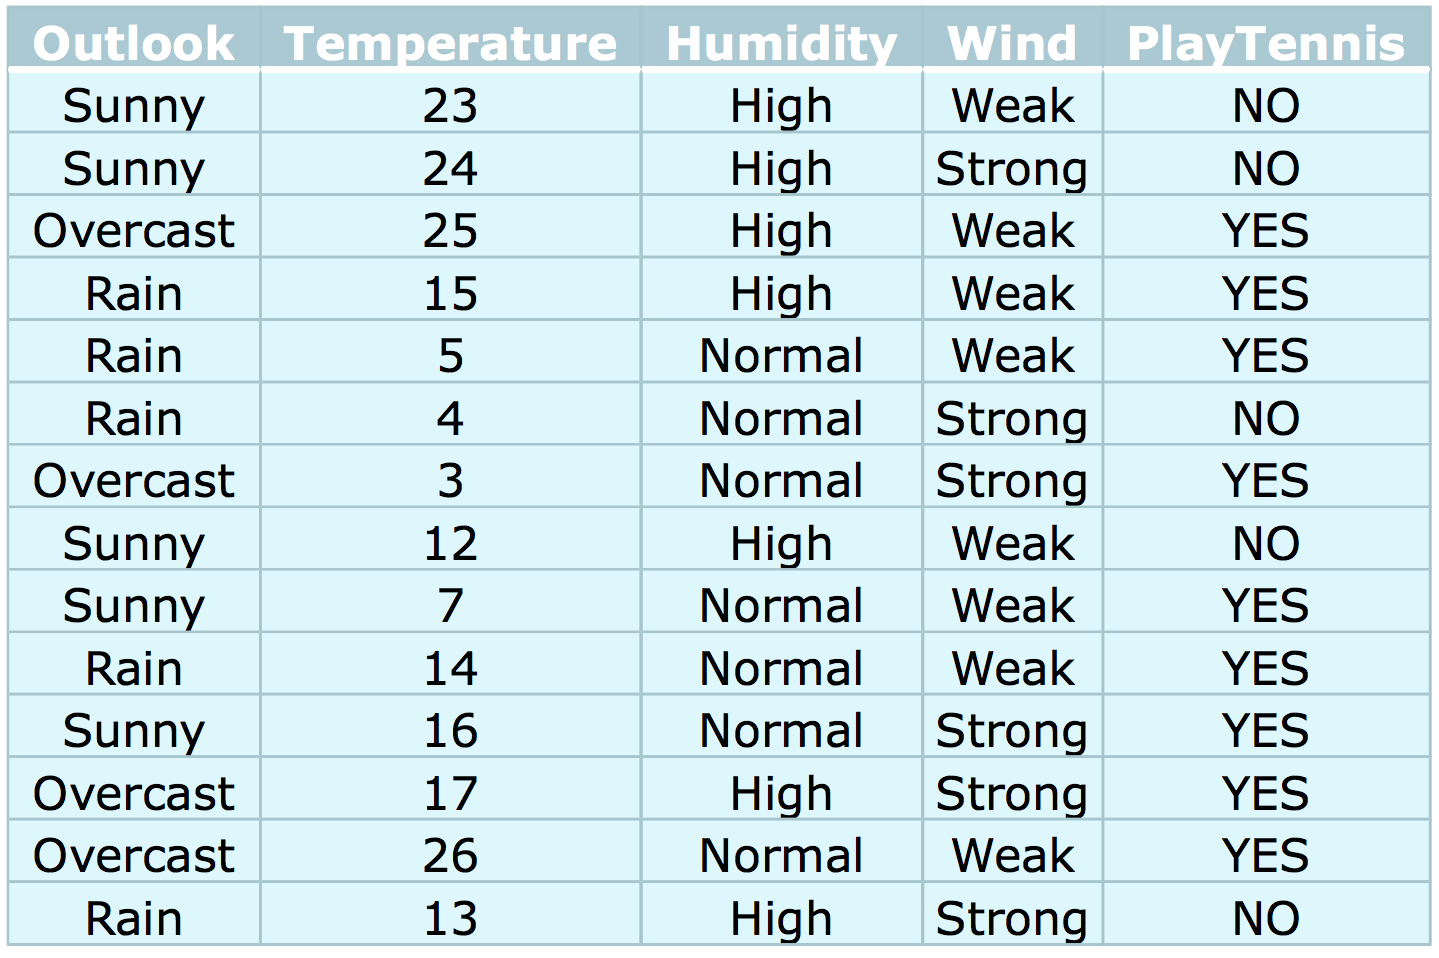
\includegraphics[width=0.5\textwidth]{table-exercise-6}
				\caption{Datos para el algoritmo J48}
			\end{center}
		\end{table}

		\paragraph{}

%-----------------------------
%	BIBLIOGRAPHY
%-----------------------------
	\nocite{subject:taa}
	\bibliographystyle{acm}
  \bibliography{bib/misc}

\end{document}
